\begin{appendices}


\chapter{RDF-Doctor Grammar}
\label{ch:appendix}

% Applies only when you use it
\lstset{
    basicstyle=\color{blue},%
    breaklines=true,%                                      allow line breaks
    moredelim=[s][\color{green!50!black}\ttfamily]{'}{'},% single quotes in green
    moredelim=*[s][\color{black}\ttfamily]{options}{\}},%  options in black (until trailing })
    commentstyle={\color{gray}\itshape},%                  gray italics for comments
    morecomment=[l]{//},%                                  define // comment
    emph={%
        STRING%                                            literal strings listed here
        },emphstyle={\color{blue}\ttfamily},%              and formatted in blue
    alsoletter={:,|,;},%
    morekeywords={:,|,;},%                                 define the special characters
    keywordstyle={\color{black}},%                         and format them in black
}

\begin{lstlisting}
grammar Turtle;

@parser::members { // add members to check Namespace declaration
	public List<String> symbols = new ArrayList<String>();
	boolean isExistNS(String in ) { // custom constructor
		boolean foundNS = false ; 
		for(String s : symbols ){
			if(s.contains(in.split(":")[0])){
				foundNS = true; 
				break;
			}
		}
		return foundNS;
	}
}

start
: statement*  EOF
;

statement
: directive
| triples '.'
| triples ',' {notifyErrorListeners("Bad end of a triple with ','");}
| triples ';' {notifyErrorListeners("Bad end of a triple with ';'");}
| triples {notifyErrorListeners("Missing '.' at the end of a triple");}
| triples ('.')+ ('.')+ {notifyErrorListeners("Too many DOT");}
| errors		

;

directive
//	/* List of symbols defined within this block */
//	locals [
//	]
: sparqlPrefix
| sparqlBase 
| prefixID    //{System.out.println("symbols="+$symbols);}
| base
| unkonwnDecl
| sparqlPrefix '.' {notifyErrorListeners("Extraneous '.' at the end of SPARQL prefix directive");}
| sparqlBase '.' {notifyErrorListeners("Extraneous '.' at the end of SPARQL base directive");}
;

errors	
: iri '=' iri '.' {notifyErrorListeners("'=' sign cannot be used in Turtle");}
| iri '<=' iri '.'  {notifyErrorListeners("'<=' symbol cannot be used in Turtle");}
| iri '=>' iri '.'  {notifyErrorListeners("'=>' symbol cannot be used in Turtle");}
////TODO:time much time
////    | subject predicate object graphLabel? '.' {notifyErrorListeners("Turtle is not NQOUDS");}
////TODO
//// 	| BAD_PNAME_LN_ENDS_WITH_DOT BAD_PNAME_LN_ENDS_WITH_DOT  BAD_PNAME_LN_ENDS_WITH_DOT  {notifyErrorListeners("'IRI' as a Subject or a Predicate cannot be followed by '.' in Turtle");}
| (iri '.')+ (iri '.')+  triples '.' {notifyErrorListeners("N3 paths cannot be used in Turtle");}
| (iri '.')+ (iri '.')+  triples  {notifyErrorListeners("N3 paths cannot be used in Turtle");}
| '@forAll' iri '.' {notifyErrorListeners(" '@forAll' cannot be used in Turtle ");}
| '@forSome' iri '.' {notifyErrorListeners(" '@forSome' cannot be used in Turtle ");}
| ('a'|CHARS)* '@a' ('a'|CHARS)* '.' {notifyErrorListeners(" '@a' cannot be used in Turtle ");}
;


graphLabel
: 	IRIREF | BLANK_NODE_LABEL
;

unkonwnDecl 	:
'@keywords' ('a'|CHARS)*  '.' {notifyErrorListeners("@keywords is unkown directive in Turtle");}
;	

prefixID
:
'@prefix' CHARS '.' ':' IRIREF '.' {notifyErrorListeners("Prefix Namespace cannot end with '.' ");}
| '@prefix' '.' CHARS ':' IRIREF '.' {notifyErrorListeners("Prefix Namespace cannot start with '.' ");}
| '@prefix' ':' IRIREF '.' 
| '@prefix' PNAME_NS IRIREF '.' {symbols.add($PNAME_NS.text);} // { System.out.println($PNAME_NS.text + $IRIREF.text);} 
//  | '@prefix' (PN_PREFIX)? ':' IRIREF '.' { System.out.println($PN_PREFIX.text + $IRIREF.text);} 
| '@prefix' PNAME_NS IRIREF ('.')+ ('.')+ {notifyErrorListeners("Too many DOT ");}
| PNAME_NS IRIREF '.' {notifyErrorListeners("Missing Prefix keyword, use '@prefix'");}
| '@prefix'   IRIREF '.' {notifyErrorListeners("Missing NameSpace in Prefix directive");}
| '@prefix' CHARS*  IRIREF '.'  {notifyErrorListeners("Missing ':' in Prefix directive");}
;

//   | '@prefix' PNAME_NS IRIREF {notifyErrorListeners("Missing '.' at the end of Prefix directive");}
//   | '@prefix' PNAME_NS  '.' {notifyErrorListeners("Missing IRI in Prefix directive");}
//   | '@prefix' PNAME_NS  {notifyErrorListeners("Missing IRI  and dot at Prefix directive");}


base
: '@base' IRIREF '.'
| '@base' IRIREF ('.')+ ('.')+ {notifyErrorListeners("Too many DOT ");}
;

sparqlBase
: KW_BASE  IRIREF 
| '@BASE'   IRIREF '.'  {notifyErrorListeners("incorrect syntax form of base directive");}
;

sparqlPrefix
: KW_PREFIX CHARS '.' ':' IRIREF  {notifyErrorListeners("Prefix Namespace cannot end with '.' ");}
| KW_PREFIX '.' CHARS ':' IRIREF  {notifyErrorListeners("Prefix Namespace cannot start with '.' ");}
| KW_PREFIX PNAME_NS IRIREF
| KW_PREFIX ':' IRIREF
| PNAME_NS IRIREF {notifyErrorListeners("Missing Prefix keyword, use 'PREFIX'");}
| KW_PREFIX  IRIREF  {notifyErrorListeners("Missing NameSpace in Prefix directive");}
;

KW_BASE : B A S E ;
KW_PREFIX : P R E F I X ;

triples
:    
subject predicateObjectList
| blankNodePropertyList predicateObjectList?
| subject ':' object 
| subject verb {notifyErrorListeners("Object of a triple is missing");}
;

predicateObjectList
: verb objectList (';' (verb objectList)?)*
;

objectList
: object (',' object)*
;

verb
: predicate
| 'is' predicate 'of' {notifyErrorListeners("'is .. of' pattern is not used in Turtle");}
| 'a'
| 'A' {notifyErrorListeners("'A' cannot be used as predicate, it should be repalced with 'a'");}
| BooleanLiteral {notifyErrorListeners("Predicate cannot be a boolean value");}
| NumericLiteral  {notifyErrorListeners("Predicate cannot be a number");}
| literal {notifyErrorListeners("Predicate cannot be a literal");}
| BlankNode {notifyErrorListeners("Predicate cannot be a blank node");}
;

subject
: iri
| BlankNode
| BlankNode  '.' {notifyErrorListeners("Blank Node cannot be followed by '.'");}
| 'a' {notifyErrorListeners("'a' cannot be used as a subject");}
| BooleanLiteral {notifyErrorListeners("Subject cannot be a boolean value");}
| NumericLiteral  {notifyErrorListeners("Subject cannot be a number");}
| rdfLiteral   {notifyErrorListeners("Subject cannot be a string");}

| collection
| '{' triples '.' '}' {notifyErrorListeners("{ } pattern cannot be used in Turtle");}
| '{' triples '}' {notifyErrorListeners("{ } pattern cannot be used in Turtle");} 
// todo
//				| rdfLiteral   {notifyErrorListeners("Subject cannot be a string");}

;

predicate
: iri
;

object
: iri
| BlankNode
| collection
| blankNodePropertyList
| badBlankNodePropertyList  {notifyErrorListeners("incorrect form of a blank node list");}
| literal
| 'a' {notifyErrorListeners("'a' cannot be used as an object");}
;

literal
: rdfLiteral
| NumericLiteral
| BooleanLiteral
| BadLiteral {notifyErrorListeners("incorrect form of a Literal");}
;

blankNodePropertyList
: '[' predicateObjectList ']'
;
//TODO: if this only for number or for every object
badBlankNodePropertyList   
: '[' predicateObjectList '.' ']'
;
collection
: '(' object* ')'
;


NumericLiteral
: INTEGER | DECIMAL | DOUBLE
;

rdfLiteral
: 
BAD_STRING_LITERAL_LONG_QUOTE_TOO_MANY (LANGTAG | '^^' iri)? {notifyErrorListeners("incorrect form of long literal with 4 qoutes");}
| BAD_STRING_LITERAL_LONG_SINGLE_QUOTE_TOO_MANY (LANGTAG | '^^' iri)? {notifyErrorListeners("incorrect form of long literal with 4 qoutes");}
| String (LANGTAG | '^^' iri)?
| String  BAD_LANGTAG_AS_NUMBER  {notifyErrorListeners("Language tag cannot be a numeric value");}
| String '^' iri {notifyErrorListeners("Missing '^' Character");}
| String LANGTAG '^^' iri {notifyErrorListeners("incorrect form of a Literal");}
| String '^^' iri LANGTAG {notifyErrorListeners("incorrect form of a Literal");}  
| (BAD_STRING_LITERAL_LONG_SINGLE_QUOTE | BAD_STRING_LITERAL_LONG_QUOTE ) (LANGTAG | '^^' iri)?  {notifyErrorListeners("incorrect quotes of a literal");}
| BAD_STRING_LITERAL_SINGLE_QUOTE (LANGTAG | '^^' iri)? {notifyErrorListeners("incorrect quotes of a literal");}
| BAD_STRING_LITERAL_QUOTE (LANGTAG | '^^' iri)? {notifyErrorListeners("incorrect quotes of a literal");}
| (BAD_STRING_LITERAL_QUOTE_WITH_BAD_UCHAR | BAD_STRING_LITERAL_SINGLE_QUOTE_WITH_BAD_UCHAR | BAD_STRING_LITERAL_LONG_SINGLE_QUOTE_WITH_BAD_UCHAR | BAD_STRING_LITERAL_LONG_QUOTE_WITH_BAD_UCHAR) {notifyErrorListeners("Bad Unicode Characters, Only HEX Characters are allowed");}
| (BAD_STRING_LITERAL_QUOTE_WITH_BAD_ESCAPE | BAD_STRING_LITERAL_SINGLE_QUOTE_WITH_BAD_ESCAPE | BAD_STRING_LITERAL_LONG_SINGLE_QUOTE_WITH_BAD_ESCAPE | BAD_STRING_LITERAL_LONG_QUOTE_WITH_BAD_ESCAPE) {notifyErrorListeners("Bad Literal Escape");}
//   |   {notifyErrorListeners("Uncorrect form of long literal with 4 qoutes");}
;


BooleanLiteral
: 'true' | 'false'
;

BadLiteral 
: NumericLiteral ('.')+ CHARS 
| NumericLiteral CHARS 
;

String
: 
STRING_LITERAL_QUOTE | STRING_LITERAL_SINGLE_QUOTE | STRING_LITERAL_LONG_SINGLE_QUOTE | STRING_LITERAL_LONG_QUOTE

;

iri
: 
IRIREF 
|  PrefixedName { if(!isExistNS($PrefixedName.text))notifyErrorListeners($PrefixedName.text.split(":")[0] +" prefix is undefined ");}
//	 | PNAME_LN | (PN_PREFIX)? ':'   
//      	{
	//	if ( !$directive:symbols.contains($PN_PREFIX.text) ) {
		//	System.err.println("Undefined prefix: "+PN_PREFIX.text);
		//	}
	//	}
//ToDO   
// | PNAME_NS  PN_LOCAL_BAD_WITH_DASH {notifyErrorListeners("Bad syntax of Prefixed IRI, the local prefix namespace cannot start with dash");}
| PNAME_NS  BAD_PN_LOCAL_STARTS_WITH_PERCENT {notifyErrorListeners("Bad syntax of Prefixed IRI, the local prefix namespace cannot contain '%'");}
	//   | PNAME_NS  PN_LOCAL_BAD_WITH_PERCENT {notifyErrorListeners("Bad syntax of Prefixed IRI, the local prefix namespace cannot contain '%'");}
		| BAD_PNAME_LN_STARTS_WITH_DOT  {notifyErrorListeners("incorrect form of Prefixed Namespace, it cannot start with '.'");} 
		| BAD_PNAME_LN_ENDS_WITH_DOT  {notifyErrorListeners("incorrect form of Prefixed Namespace, it cannot end with '.'");} 
		| BAD_IRIREF_WITH_SPACE {notifyErrorListeners("Bad syntax of IRI, IRI cannot contain space or newline");}
		| BAD_IRIREF_WITH_MULTIPLE_ANGLE_BRACKETS {notifyErrorListeners("Bad syntax of IRI, Too many angle brackets in IRI");}
		| BAD_IRIREF_WITH_PARENTHESES {notifyErrorListeners("Bad syntax of IRI, IRI cannot contain parentheses");}
		;
		
		
		BlankNode
		: BLANK_NODE_LABEL 
		| ANON
		;
		
		CHARS: 
		[a-zA-Z]+ [0-9]*
		;
		
		WS
		: ([\t\r\n\u000C] | ' ') + -> skip
		;
		
		COMMENT				  
		: '#' ~[\r\n]* -> skip;
		// LEXER
		
		PN_PREFIX
		: PN_CHARS_BASE ((PN_CHARS | '.')* PN_CHARS)?
		;
		
		//IRIREF	        :	'<' (~(['\u0000'..'\u0020']|'<'|'>'|'"'|'{'|'}'|'|'|'^'|'`'|'\\') | UCHAR)* '>'; /* \u00=NULL #01-\u1F=control codes \u20=space */
		
		IRIREF
		:
		'<' (~[\u0000-\u0020<>"{}|^`\\] | UCHAR)* '>' 
		
		;
		
		
		PNAME_NS
		: PN_PREFIX? ':'
		;
		
		
		PrefixedName
		: PNAME_LN | PNAME_NS
		;
		
		
		PNAME_LN
		: PNAME_NS PN_LOCAL?
		;
		
		BAD_PNAME_LN_STARTS_WITH_DOT	  
		: '.' PN_PREFIX ':' PN_LOCAL 
		;
		
		BAD_PNAME_LN_ENDS_WITH_DOT	  
		: PN_PREFIX  '.:' PN_LOCAL 
		;
		
		BLANK_NODE_LABEL
		: '_:' (PN_CHARS_U | [0-9]) ((PN_CHARS | '.')* PN_CHARS)?
		;
		
		
		LANGTAG
		: '@' [a-zA-Z] + ('-' [a-zA-Z0-9] +)*
		;
		
		BAD_LANGTAG_AS_NUMBER
		: '@' [0-9]+
		;
		
		INTEGER
		: [+-]? [0-9] +
		;
		
		
		DECIMAL
		: [+-]? [0-9]* '.' [0-9] +
		;
		
		
		DOUBLE
		: [+-]? ([0-9] + '.' [0-9]* EXPONENT | '.' [0-9] + EXPONENT | [0-9] + EXPONENT)
		;
		
		
		EXPONENT
		: [eE] [+-]? [0-9] +
		;
		
		
		STRING_LITERAL_LONG_SINGLE_QUOTE
		: '\'\'\'' (~[\u0027\u005C\u000A\u000D] | ECHAR | UCHAR  | '\n' )*  ('\'' | '\'\'')?  (~[\u0027\u005C\u000A\u000D] | ECHAR | UCHAR)* '\'\'\''  
		;
		
		
		STRING_LITERAL_LONG_QUOTE
		: '"""'  ((~ ["\\] | ECHAR | UCHAR | '\'') ('"' | '""')? (~ ["\\] | ECHAR | UCHAR | '\''))* '"""'
		;
		
		STRING_LITERAL_QUOTE
		: '"' (~[\u0022\u005C\u000A\u000D] | ECHAR | UCHAR)* '"' 
		;
		
		STRING_LITERAL_SINGLE_QUOTE
		: '\'' (~ [\u0027\u005C\u000A\u000D] | ECHAR | UCHAR | '"')* '\''
		;
		
		BAD_STRING_LITERAL_QUOTE_WITH_BAD_UCHAR
		: '"' (~[\u0022\u005C\u000A\u000D] | ECHAR | UCHAR)* BAD_UCHAR (~[\u0022\u005C\u000A\u000D] | ECHAR | UCHAR)* '"' 
		;
		
		BAD_STRING_LITERAL_SINGLE_QUOTE_WITH_BAD_UCHAR
		: '\'' (~ [\u0027\u005C\u000A\u000D] | ECHAR | UCHAR | '"')*  BAD_UCHAR (~ [\u0027\u005C\u000A\u000D] | ECHAR | UCHAR | '"')*  '\''
		;
		
		BAD_STRING_LITERAL_LONG_SINGLE_QUOTE_WITH_BAD_UCHAR
		: '\'\'\'' (~[\u0027\u005C\u000A\u000D] | ECHAR | UCHAR  | '\n' )*  ('\'' | '\'\'')?  (~[\u0027\u005C\u000A\u000D] | ECHAR | UCHAR)* BAD_UCHAR   (~[\u0027\u005C\u000A\u000D] | ECHAR | UCHAR  | '\n' )*  ('\'' | '\'\'')?  (~[\u0027\u005C\u000A\u000D] | ECHAR | UCHAR)*'\'\'\''  
		;
		
		BAD_STRING_LITERAL_LONG_QUOTE_WITH_BAD_UCHAR
		: '"""'  (~[\u0022\u005C\u000A\u000D] | ECHAR | UCHAR)*   BAD_UCHAR (~[\u0022\u005C\u000A\u000D] | ECHAR | UCHAR)*   '"""'
		;
		
		BAD_STRING_LITERAL_QUOTE_WITH_BAD_ESCAPE
		: '"' (~[\u0022\u005C\u000A\u000D] | ECHAR | UCHAR)* ILLEGAL_ESCAPE (~[\u0022\u005C\u000A\u000D] | ECHAR | UCHAR)* '"' 
		;
		
		BAD_STRING_LITERAL_SINGLE_QUOTE_WITH_BAD_ESCAPE
		: '\'' (~ [\u0027\u005C\u000A\u000D] | ECHAR | UCHAR | '"')*  ILLEGAL_ESCAPE (~ [\u0027\u005C\u000A\u000D] | ECHAR | UCHAR | '"')*  '\''
		;
		
		BAD_STRING_LITERAL_LONG_SINGLE_QUOTE_WITH_BAD_ESCAPE
		: '\'\'\'' (~[\u0027\u005C\u000A\u000D] | ECHAR | UCHAR  | '\n' )*  ('\'' | '\'\'')?  (~[\u0027\u005C\u000A\u000D] | ECHAR | UCHAR)* ILLEGAL_ESCAPE   (~[\u0027\u005C\u000A\u000D] | ECHAR | UCHAR  | '\n' )*  ('\'' | '\'\'')?  (~[\u0027\u005C\u000A\u000D] | ECHAR | UCHAR)*'\'\'\''  
		;
		
		BAD_STRING_LITERAL_LONG_QUOTE_WITH_BAD_ESCAPE
		: '"""'  (~[\u0022\u005C\u000A\u000D] | ECHAR | UCHAR)*   ILLEGAL_ESCAPE (~[\u0022\u005C\u000A\u000D] | ECHAR | UCHAR)*   '"""'
		;
		
		fragment UCHAR
		: '\\u' HEX HEX HEX HEX | '\\U' HEX HEX HEX HEX HEX HEX HEX HEX
		;
		
		BAD_UCHAR
		: '\\u' HEX* NONHEX+ | '\\U' HEX* NONHEX+ 
		;
		
		ECHAR
		: '\\' [tbnrf"'\\]
		;
		
		
		ANON_WS
		: ' ' | '\t' | '\r' | '\n'
		;
		
		
		ANON
		: '[' ANON_WS* ']'
		;
		
		
		PN_CHARS_BASE
		: [A-Z] | [a-z] | [\u00C0-\u00D6] | [\u00D8-\u00F6] | [\u00F8-\u02FF] | [\u0370-\u037D]
		| [\u037F-\u1FFF] | [\u200C-\u200D] | [\u2070-\u218F] | [\u2C00-\u2FEF] | [\u3001-\uD7FF]
		| [\uF900-\uFDCF] | [\uFDF0-\uFFFD]				   		   
		;
		
		
		PN_CHARS_U
		: PN_CHARS_BASE | '_'
		;
		
		
		PN_CHARS
		: PN_CHARS_U | '-' | [0-9] | '\u00B7' | [\u0300-\u036F] | [\u203F-\u2040]
		;
		
		
		PN_LOCAL
		: (PN_CHARS_U | ':' | [0-9] | PLX) ((PN_CHARS | '.' | ':' | PLX)* (PN_CHARS | ':' | PLX))?
		;
		
		
		BAD_PN_LOCAL_STARTS_WITH_PERCENT
		:   '%' PN_LOCAL
		;
		
		
		PLX
		: PERCENT | PN_LOCAL_ESC
		;
		
		
		PERCENT
		: '%' HEX HEX
		;
		
		
		HEX
		: [0-9] | [A-F] | [a-f]
		;
		
		NONHEX
		: [g-zG-Z]
		;
		
		
		PN_LOCAL_ESC
		: '\\' ('_' | '~' | '.' | '-' | '!' | '$' | '&' | '\'' | '(' | ')' | '*' | '+' | ',' | ';' | '=' | '/' | '?' | '#' | '@' | '%')
		;
		
		
		
		
		
		// check if the IRI has a newline or space  
		BAD_IRIREF_WITH_SPACE
		:  '<' (PN_CHARS | '.' | ':' | '/' | '\\' | '#' | '@' | '%' | '&' | UCHAR)* '\n>'
		| '<' (PN_CHARS | '.' | ':' | '/' | '\\' | '#' | '@' | '%' | '&' | UCHAR)* '\u0020>'
		| '<' (PN_CHARS | '.' | ':' | '/' | '\\' | '#' | '@' | '%' | '&' | UCHAR)* ANON_WS+ (PN_CHARS | '.' | ':' | '/' | '\\' | '#' | '@' | '%' | '&' | UCHAR)*'>'
		
		;
		BAD_IRIREF_WITH_MULTIPLE_ANGLE_BRACKETS
		:'<' (PN_CHARS | '.' | ':' | '/' | '\\' | '#' | '@' | '%' | '&' | UCHAR)* '\u003C>'
		| '<' (PN_CHARS | '.' | ':' | '/' | '\\' | '#' | '@' | '%' | '&' | UCHAR)* '\u003E>'
		;
		BAD_IRIREF_WITH_PARENTHESES 
		: '<' (PN_CHARS | '.' | ':' | '/' | '{'| '}' | '\\' | '#' | '@' | '%' | '&' | UCHAR)* '>'
		;
		
		BAD_STRING_LITERAL_SINGLE_QUOTE   
		: '\'\'\'' (~[\u0027\u005C\u000A\u000D] | ECHAR | UCHAR)* '\'' 
		| '\'' (~[\u0027\u005C\u000A\u000D] | ECHAR | UCHAR)* '\'\'\'' 
		;
		
		BAD_STRING_LITERAL_QUOTE      
		: '"""' (~[\u0022\u005C\u000A\u000D] | ECHAR | UCHAR)* '"' 
		| '"' (~[\u0022\u005C\u000A\u000D] | ECHAR | UCHAR)* '"""' 
		| '"' (~[\u0022\u005C\u000A\u000D] | ECHAR | UCHAR)* '\'' 
		| '\'' (~[\u0022\u005C\u000A\u000D] | ECHAR | UCHAR)* '"' 			
		;  	  
		
		BAD_STRING_LITERAL_LONG_SINGLE_QUOTE
		: '\'\'\'' (('\'' | '\'\'')? ([^'\\] | ECHAR | UCHAR | '"'))* '"""'
		;
		
		BAD_STRING_LITERAL_LONG_QUOTE
		: '"""' (('"' | '""')? (~ ["\\] | ECHAR | UCHAR | '\''))* '\'\'\''
		;
		BAD_STRING_LITERAL_LONG_QUOTE_TOO_MANY
		: '"""' (('"' | '""')? (~ ["\\] | ECHAR | UCHAR ))* '""""'
		| '""""' (('"' | '""')? (~ ["\\] | ECHAR | UCHAR ))* '"""'
		;	
		
		BAD_STRING_LITERAL_LONG_SINGLE_QUOTE_TOO_MANY
		: '\'\'\'' (~[\u0027\u005C\u000A\u000D] | ECHAR | UCHAR)*  '\'\'\'\''
		| '\'\'\'\''(~[\u0027\u005C\u000A\u000D] | ECHAR | UCHAR)*  '\'\'\''
		;
		
		
		ILLEGAL_ESCAPE
		: ('\\' ~[ubtnfr"'\\] ) [a-zA-Z]+ 
		;
		
		fragment A:('a'|'A');
		fragment B:('b'|'B');
		fragment C:('c'|'C');
		fragment D:('d'|'D');
		fragment E:('e'|'E');
		fragment F:('f'|'F');
		fragment G:('g'|'G');
		fragment H:('h'|'H');
		fragment I:('i'|'I');
		fragment J:('j'|'J');
		fragment K:('k'|'K');
		fragment L:('l'|'L');
		fragment M:('m'|'M');
		fragment N:('n'|'N');
		fragment O:('o'|'O');
		fragment P:('p'|'P');
		fragment Q:('q'|'Q');
		fragment R:('r'|'R');
		fragment S:('s'|'S');
		fragment T:('t'|'T');
		fragment U:('u'|'U');
		fragment V:('v'|'V');
		fragment W:('w'|'W');
		fragment X:('x'|'X');
		fragment Y:('y'|'Y');
		fragment Z:('z'|'Z');	


\end{lstlisting}

\chapter{RDF Syntax Errors Categories }
\label{ch:synErrCategories}


% \newcounter{cA} 
% \setcounter{cA}{1}
% \begin{longtable}{|c|p{3cm}|p{3cm}|l|l}
% \caption{\textbf{Categories of syntax errors of N-Triple and Turtle serializations.} These categories are extracted from files of Turtle Test Suite \cite{TurtleTests:Online}, including   incorrect syntactic forms.}
% \label{tab:syntaxErrorCate}
% \centering
% \cline{2-5}
% Sn. & Category & Position & Sample &  \\  
% \cline{1-4}

% \thecA     \addtocounter{cA}{1}  & \centering \multirow{3}{=}{ \textcolor{blue}{Bad String Escape}
% } & Literal & \textcolor{red}{"a\textbackslash zb" } &  \\ \cline{1-1} \cline{3-4}
% \thecA     \addtocounter{cA}{1}  &  & Literal & \textcolor{red}{"\textbackslash uWXYZ"}  &  \\ \cline{1-1} \cline{3-4}
% \thecA     \addtocounter{cA}{1}  &  & Literal &  \textcolor{red}{"\textbackslash U0000WXYZ"} &  \\   \cline{1-4}
% \thecA     \addtocounter{cA}{1}  &  \multirow{5}{=}{ \textcolor{blue}{Misuse of Keywords}} & Predicate &  :s \textcolor{red}{ A} :o . &  \\   \cline{1-1} \cline{3-4}
% \thecA     \addtocounter{cA}{1} &  & Subject &\textcolor{red}{ a} :p :o . &  \\ \cline{1-1} \cline{3-4}
% \thecA     \addtocounter{cA}{1} &  & Object & :s :p \textcolor{red}{ a} .  &  \\ \cline{1-1} \cline{3-4}
% \thecA     \addtocounter{cA}{1} &  & Subject & \textcolor{red}{true} :p :o . &  \\ \cline{1-1} \cline{3-4}
% \thecA     \addtocounter{cA}{1}  &  & Object & :s \textcolor{red}{true} :o . &  \\   \cline{1-4}
% \thecA     \addtocounter{cA}{1}  &   \textcolor{blue}{Bad Language Tag} & Language Tag &  “duck”@\textcolor{red}{1} &  \\ \cline{1-4}
% \thecA     \addtocounter{cA}{1}  &  \multirow{5}{=}{ \textcolor{blue}{Bad Local Namespace in Prefixed IRI}} & Prefixed IRI &  :s :p \textcolor{red}{ :-a}  . &  \\   \cline{1-1} \cline{3-4}
% \thecA     \addtocounter{cA}{1}  &  & Prefixed IRI & :s :p \textcolor{red}{ :o\%2} .&  \\ \cline{1-1} \cline{3-4}
% \thecA     \addtocounter{cA}{1}  &  & Prefixed IRI & :s :p \textcolor{red}{ :\%o2} .&  \\ \cline{1-1} \cline{3-4}
% \thecA     \addtocounter{cA}{1}  &  & Prefixed IRI & :s :p \textcolor{red}{:a\texttt{\~{}}b} . &  \\ \cline{1-1} \cline{3-4}
% \thecA     \addtocounter{cA}{1}  &  & Prefixed IRI &  \textcolor{red}{:a\textbackslash u0039} :p :o . &  \\   \cline{1-4}
% \thecA     \addtocounter{cA}{1}  & \multirow{2}{=}{ \textcolor{blue}{Bad Prefix Label in  Prefixed IRI}
% } & Prefixed IRI & :s :p \textcolor{red}{ ex.}:o . &  \\ \cline{1-1} \cline{3-4}
% \thecA     \addtocounter{cA}{1}  &  & Prefixed IRI & :s :p \textcolor{red}{.ex}:o .  &  \\ \cline{1-4}
% \thecA     \addtocounter{cA}{1}  &  \multirow{5}{=}{ \textcolor{blue}{Bad Syntax from N3 Notation }} & Curly Brackets & \textcolor{red}{ \{ :a :q :c . \}}  :p :o . &  \\   \cline{1-1} \cline{3-4}
% \thecA     \addtocounter{cA}{1}  &  & Equal Sign & :a \textcolor{red}{ =} :b .&  \\ \cline{1-1} \cline{3-4}
% \thecA     \addtocounter{cA}{1}  &  & N3 Paths & \textcolor{red}{ :x.
%   ns:p.
%     ns:q } :p :z . &  \\ \cline{1-1} \cline{3-4}
% \thecA     \addtocounter{cA}{1}  &  & N3 Paths & \textcolor{red}{:x\textasciicircum ns:p } :p :z . &  \\ \cline{1-1} \cline{3-4}
% \thecA     \addtocounter{cA}{1}  &  & ‘is .. of’ Pattern & :z \textcolor{red}{ is}  :p \textcolor{red}{ of}  :x .  \\ \cline{1-1} \cline{3-4}
% \thecA     \addtocounter{cA}{1}  & &  {IRIs without Space}& \textcolor{red}{ :a.:b.:c } . &  \\ \cline{1-1} \cline{3-4}
% \thecA     \addtocounter{cA}{1}  &  & '@keywords'  & \textcolor{red}{@keywords  
% } a .  \\ & & Pattern &   a Item . &  \\\cline{1-1} \cline{3-4}
% \thecA     \addtocounter{cA}{1}  &  & '@keywords' & \textcolor{red}{@keywords  
% }  . \\ & & Pattern & 
% x \textcolor{red}{@a} Item .  &  \\\cline{1-1} \cline{3-4}
% \thecA     \addtocounter{cA}{1}  &  & '\textless=' Pattern & :s \textcolor{red}{ \textless=} :o .&  \\ \cline{1-1} \cline{3-4}
% \thecA     \addtocounter{cA}{1}  &  & '=\textgreater' Pattern  & :s   \textcolor{red}{ =\textgreater} :o  .&  \\ \cline{1-1} \cline{3-4}
% \thecA     \addtocounter{cA}{1}  &  &'@forSome' Pattern & \textcolor{red}{@forSome } :x .  \\ \cline{1-1} \cline{3-4}
% \thecA     \addtocounter{cA}{1}  &  & '@forAll' Pattern  & \textcolor{red}{@forAll } :x .   \\  \cline{1-4}
% \thecA     \addtocounter{cA}{1}  & \multirow{2}{=}{ \textcolor{blue}{Bad Prefix Label in Directives}
% } & \multirow{2}{=}{Directive} & @prefix  \textcolor{red}{eg.} :\textless example\textgreater . \\ & &  & \textcolor{red}{eg.}:s  :p  :o  . &  \\\cline{1-1} \cline{3-4}
% \thecA     \addtocounter{cA}{1}  &   & \multirow{2}{*}{Directive} & @prefix   \textcolor{red}{.eg} :\textless example\textgreater . \\ & &  & \textcolor{red}{.eg}:s  :p  :o . &  \\ \cline{1-4}
% \thecA     \addtocounter{cA}{1}  &  \multirow{5}{=}{ \textcolor{blue}{Bad Number as a Literal:}} & Literal &  :s :p  \textcolor{red}{ 123.abc}  . &  \\   \cline{1-1} \cline{3-4}
% \thecA     \addtocounter{cA}{1}  &  & Literal & :s :p \textcolor{red}{ 123e} .&  \\ \cline{1-1} \cline{3-4}
% \thecA     \addtocounter{cA}{1}  &  & Literal & :s :p \textcolor{red}{ 123abc} .&  \\ \cline{1-1} \cline{3-4}
% \thecA     \addtocounter{cA}{1}  &  & Literal & :s :p \textcolor{red}{0x123} . &  \\ \cline{1-1} \cline{3-4}
% \thecA     \addtocounter{cA}{1}  &  & Literal & :s :p  \textcolor{red}{+- 1} . &  \\   \cline{1-4}
% \thecA     \addtocounter{cA}{1}  &   \textcolor{blue}{Bad Directives} &  \multirow{2}{*}{Directive} &  \textcolor{red}{\#Missing a prefix for ':'}\\
% & & & \textcolor{red}{ :}s \textcolor{red}{ :}p  "x"  . &  \\   \cline{1-1} \cline{3-4}
%  \thecA     \addtocounter{cA}{1}  &  & \multirow{2}{*}{Directive} &   \textcolor{red}{\#Missing an IRI}\\
% & & & @prefix ex: . &  \\ \cline{1-1} \cline{3-4}
%  \thecA     \addtocounter{cA}{1}  &  & \multirow{2}{*}{Directive} &   \textcolor{red}{\#Missing a prefix label}\\
% & & &@prefix \textless example\textgreater . &  \\ & & &  \\   \cline{1-1} \cline{3-4}
%  \thecA     \addtocounter{cA}{1}  &  & \multirow{2}{*}{Directive} &   \textcolor{red}{\#Missing a colon }\\
% & & & @prefix ex \textless example\textgreater . &  \\   \cline{1-4}
% \thecA     \addtocounter{cA}{1}  &  \multirow{8}{*}{ \textcolor{blue}{Bad String}} & Literal &  :s :p \textcolor{red}{ "abc' }. &  \\   \cline{1-1} \cline{3-4}
% \thecA     \addtocounter{cA}{1}  &  & Literal &  :s :p \textcolor{red}{'abc"  }. &  \\ \cline{1-1} \cline{3-4}
% \thecA     \addtocounter{cA}{1}  &  & Literal &  :s :p \textcolor{red}{ '''abc' }.  &  \\ \cline{1-1} \cline{3-4}
% \thecA     \addtocounter{cA}{1}  &  & Literal &  :s :p \textcolor{red}{ """abc'''  }. &  \\ \cline{1-1} \cline{3-4}
% \thecA     \addtocounter{cA}{1}  &  & Literal &  :s :p \textcolor{red}{ """abc }. &  \\ \cline{1-1} \cline{3-4}
% \thecA     \addtocounter{cA}{1}  &  & Literal &  :s :p \textcolor{red}{ """abc""""@en }. &  \\ \cline{1-1} \cline{3-4}
% \thecA     \addtocounter{cA}{1}  &  & Literal &  :s :p \textcolor{red}{ '''abc''''@en} . &  \\ \cline{1-1} \cline{3-4}
% \thecA     \addtocounter{cA}{1}  &  & Literal &  :s :p \textcolor{red}{ "abc"@en\textasciicircum \textasciicircum xsd:String }. &  \\   \cline{1-4}
% \thecA     \addtocounter{cA}{1}  &  \multirow{1}{=}{ \textcolor{blue}{Bad Structure }} & Nquads & \multirow{1}{*}{\textcolor{red}{ \textless s\textgreater  \textless p\textgreater  \textless o\textgreater  \textless g\textgreater } . }\\ & &  Pattern &  \\   \cline{1-1} \cline{3-4}
% \thecA     \addtocounter{cA}{1}  &  & Subject & \textcolor{red}{ “Hello”} :p :o .&  \\ \cline{1-1} \cline{3-4}
% \thecA     \addtocounter{cA}{1}  &  & Predicate & :s \textcolor{red}{ “Hello”} :o .&  \\ \cline{1-1} \cline{3-4}
% \thecA     \addtocounter{cA}{1}  &  & Predicate & :s \texttt{\textcolor{red}{[ ]}} :o . &  \\ \cline{1-1} \cline{3-4}
% \thecA     \addtocounter{cA}{1}  &  & Predicate & :s \textcolor{red}{ \_:blank} :o .&  \\ \cline{1-1} \cline{3-4}
% \thecA     \addtocounter{cA}{1}  &  & Triple &  \textcolor{red}{ \#Missing dot at the triple end} \\ & &  &  :s  :p  :o&  \\ \cline{1-1} \cline{3-4}
% \thecA     \addtocounter{cA}{1}  &  & Triple & :s  :p  :o .\textcolor{red}{.. } &  \\ \cline{1-1} \cline{3-4}
% \thecA     \addtocounter{cA}{1}  &  & Triple & :s   :p  :o \textcolor{red}{; } &  \\ \cline{1-1} \cline{3-4}
% \thecA     \addtocounter{cA}{1}  &  & Triple &  \textcolor{red}{ \#Missing an object in a triple} \\ & &  & :s :p  .&    \\   \cline{1-4}
% \thecA     \addtocounter{cA}{1}  &  \multirow{1}{*}{ \textcolor{blue}{Bad IRI}} &  IRI & \textless
%  http:// space\textgreater { a}  :o . &  \\   \cline{1-1} \cline{3-4}
% \thecA     \addtocounter{cA}{1}  &  &  IRI &  \textless http://\textcolor{red}{\texttt{\textbackslash u00ZZ11}}\textgreater { :p}  :o .&  \\ \cline{1-1} \cline{3-4}
% \thecA     \addtocounter{cA}{1}  &  &  IRI & \textless http://\textcolor{red}{\texttt{\textbackslash U00ZZ1111}}\textgreater { :p}  :o .&  \\ \cline{1-1} \cline{3-4}
% \thecA     \addtocounter{cA}{1}  &  &  IRI & \textless http:// \\ &  &  & \textgreater { :p}  :o . &  \\ \cline{1-1} \cline{3-4}
% \thecA     \addtocounter{cA}{1}  &  &  IRI &  \textless http://\textcolor{red}{\texttt{\textbackslash}}\textgreater { :p}  :o . &   \\  \cline{1-4}
 
% \end{longtable}

 \begin{table}[H]
 	\caption{\textbf{Categories of syntax errors of N-Triple and Turtle serializations.} These categories are extracted from files of Turtle Test Suite \cite{TurtleTests:Online}, including   incorrect syntactic forms.}
 \label{tab:syntaxErrorCate}
 	\centering
\includegraphics[width=5.5in]{images/bigTable.pdf}
\end{table}

\includepdf[pages=2-3,pagecommand={},width=\textwidth,noautoscale=true,offset=80 30]{images/bigTable.pdf}
%\begin{figure}
% \centering 
% \includegraphics[scale=0.7,angle=0]{i%mages/bigTable.pdf}
%\end{figure}
\end{appendices}
